\documentclass[11pt,a4paper]{article}

% ------------------------------------------------------------------
% Mechanical Copilot -- Concepts & Architecture Guide
% Self-study document: every concept is explained in plain language
% first, then connected to the exact code in this repository.
% Compile:  pdflatex concepts_guide.tex   (twice, for the TOC)
% ------------------------------------------------------------------

\usepackage[margin=2.2cm]{geometry}
\usepackage{amsmath}
\usepackage{tikz}
\usetikzlibrary{shapes.geometric, arrows.meta, positioning, fit, backgrounds}
\usepackage{enumitem}
\usepackage{xcolor}
\usepackage{hyperref}
\usepackage{booktabs}
\usepackage{longtable}
\usepackage{fancyhdr}
\usepackage{titlesec}

\hypersetup{colorlinks=true, linkcolor=blue!60!black, urlcolor=blue!60!black}

\definecolor{layman}{RGB}{0,102,153}
\definecolor{codebox}{RGB}{30,30,40}
\definecolor{softgray}{RGB}{245,245,248}

\newcommand{\layman}[1]{\par\medskip\noindent\textcolor{layman}{\textbf{In plain words:}} #1\par\smallskip}
\newcommand{\codefile}[1]{\texttt{\small #1}}

\pagestyle{fancy}
\fancyhf{}
\fancyhead[L]{\small Mechanical Copilot -- Concepts Guide}
\fancyhead[R]{\small\thepage}

\title{\vspace{-1cm}\textbf{AI Copilot for Manufacturing Process Planning\\\& Quality Inspection}\\[4pt]
\large Concepts, Architecture \& Flowcharts -- A Learning Guide}
\author{Prepared as a self-study companion to the codebase}
\date{September 2026}

\begin{document}
\maketitle
\thispagestyle{empty}

\begin{abstract}
\noindent This guide explains \emph{every concept} used to build the AI Manufacturing
Copilot -- retrieval-augmented generation (RAG), embeddings, vector search, structured
LLM output, deterministic validation, vision inspection, human-in-the-loop workflows,
JWT authentication, and more -- each in layman's terms first, then mapped to the actual
files in this repository, with flowcharts. Read it end-to-end and you will understand
not just \emph{what} the system does, but \emph{why} each piece exists and \emph{where}
it lives in the code.
\end{abstract}

\tableofcontents
\newpage

% ==================================================================
\section{The Big Picture: What Are We Building and Why?}
% ==================================================================

\subsection{The problem, in a story}
Imagine a factory that makes precision shafts. When a customer orders 25 shafts of a new
type, a senior process engineer must write a \textbf{process plan}: an ordered list of
machining operations (turn, mill, drill, grind\dots), the machine and tools for each,
cutting speeds, and the quality checks. This knowledge lives in the heads of a few
veterans and in scattered PDFs -- SOPs, routing sheets, quality standards, past
lessons-learned. Meanwhile, quality inspectors photograph parts and judge defects by
eye, and their findings sit in a separate system nobody cross-references.

\layman{The company's expertise is locked in silos: people, PDFs, and photos. New or
busy engineers can't easily reuse it, and quality data never feeds back into planning.
The result: slow planning, repeated mistakes, defects escaping to customers.}

\subsection{The solution}
Build a \textbf{copilot} (an assistant, not an autopilot) that:
\begin{enumerate}[nosep]
  \item \textbf{Reads the plant's knowledge} (SOPs, routings, standards, lessons) and
        can answer questions about it \emph{with citations} -- this is RAG.
  \item \textbf{Drafts process plans} from part requirements, grounded in that
        knowledge, and \emph{validates them with deterministic rules}.
  \item \textbf{Inspects part images} with a vision model, but only after the image
        passes a strict quality gate.
  \item \textbf{Never ships anything on its own} -- an engineer must approve every
        plan and disposition every part, and every action is audit-logged.
\end{enumerate}

\subsection{System flowchart (the 10,000-meter view)}

\begin{center}
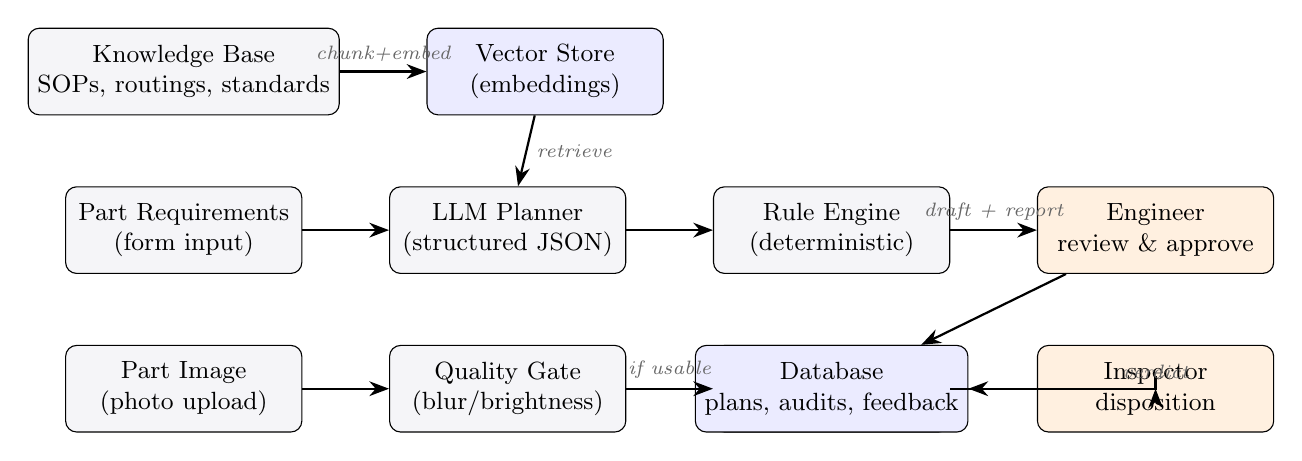
\begin{tikzpicture}[
  node distance=9mm and 11mm,
  box/.style={draw, rounded corners, fill=softgray, minimum width=30mm, minimum height=11mm, align=center, font=\small},
  store/.style={box, fill=blue!8},
  human/.style={box, fill=orange!12},
  arrow/.style={-{Stealth[length=2.5mm]}, thick},
  lab/.style={font=\scriptsize\itshape, text=black!60}
]
  \node[box] (kb) {Knowledge Base\\SOPs, routings, standards};
  \node[store, right=of kb] (vs) {Vector Store\\(embeddings)};
  \node[box, below=of kb] (req) {Part Requirements\\(form input)};
  \node[box, right=of req] (llm) {LLM Planner\\(structured JSON)};
  \node[box, right=of llm] (rules) {Rule Engine\\(deterministic)};
  \node[human, right=of rules] (eng) {Engineer\\review \& approve};
  \node[box, below=of req] (img) {Part Image\\(photo upload)};
  \node[box, right=of img] (gate) {Quality Gate\\(blur/brightness)};
  \node[box, right=of gate] (vlm) {VLM\\defect analysis};
  \node[human, below=of eng] (insp) {Inspector\\disposition};
  \node[store, below=of rules] (db) {Database\\plans, audits, feedback};

  \draw[arrow] (kb) -- node[lab, above]{chunk+embed} (vs);
  \draw[arrow] (vs) -- node[lab, right]{retrieve} (llm);
  \draw[arrow] (req) -- (llm);
  \draw[arrow] (llm) -- (rules);
  \draw[arrow] (rules) -- node[lab, above]{draft + report} (eng);
  \draw[arrow] (img) -- (gate);
  \draw[arrow] (gate) -- node[lab, above]{if usable} (vlm);
  \draw[arrow] (vlm) -| node[lab, near end, above]{verdict} (insp);
  \draw[arrow] (eng) -- (db);
  \draw[arrow] (insp) -- (db);
\end{tikzpicture}
\end{center}

\subsection{Where everything lives}

\begin{center}
\begin{tabular}{@{}ll@{}}
\toprule
\textbf{Concern} & \textbf{Code} \\
\midrule
Settings (all knobs) & \codefile{backend/app/core/config.py} \\
Database tables & \codefile{backend/app/models.py} \\
API request/response shapes & \codefile{backend/app/schemas.py} \\
Chunking & \codefile{backend/app/services/chunker.py} \\
Embeddings (real + offline) & \codefile{backend/app/services/embeddings.py} \\
Vector store & \codefile{backend/app/services/vector\_store.py} \\
Retrieval + citations & \codefile{backend/app/services/knowledge.py} \\
LLM gateway & \codefile{backend/app/services/llm.py} \\
Plan generation & \codefile{backend/app/services/planner.py} \\
Rule validation & \codefile{backend/app/services/rules.py} \\
Image quality gate + VLM & \codefile{backend/app/services/inspection.py} \\
Q\&A with refusal & \codefile{backend/app/services/qa.py} \\
Auth + JWT & \codefile{backend/app/core/security.py}, \codefile{app/api/deps.py} \\
API routes & \codefile{backend/app/api/routes/*.py} \\
Frontend pages & \codefile{frontend/src/pages/*.tsx} \\
Rule packs (editable by engineers) & \codefile{data/rulepacks/*.yaml} \\
\bottomrule
\end{tabular}
\end{center}

% ==================================================================
\section{Retrieval-Augmented Generation (RAG)}
% ==================================================================

\subsection{The concept}
An LLM is a brilliant intern with \emph{amnesia}: it read the whole internet during
training, but it has never seen \emph{your} SOPs, and it will confidently make things
up when unsure. \textbf{RAG} fixes this: \emph{before} asking the model to answer,
you \emph{retrieve} relevant passages from your own documents and paste them into the
prompt with one instruction: ``answer using ONLY these passages, and cite them.''

\layman{Instead of asking a know-it-all stranger, you hand the expert the relevant
manual pages \emph{open at the right page}, and ask them to answer while pointing at
the page for every claim. If the answer isn't on those pages, they must say so.}

\subsection{Why this kills hallucination (mostly)}
\begin{itemize}[nosep]
  \item The model isn't recalling -- it's \emph{reading}. Invention becomes unnecessary.
  \item Every statement can be tied to a chunk ID the user can click and verify.
  \item If retrieval finds nothing relevant, the system \emph{refuses} rather than
        guesses (see \S\ref{sec:refusal}).
\end{itemize}

\subsection{The RAG pipeline in this codebase}

\begin{center}
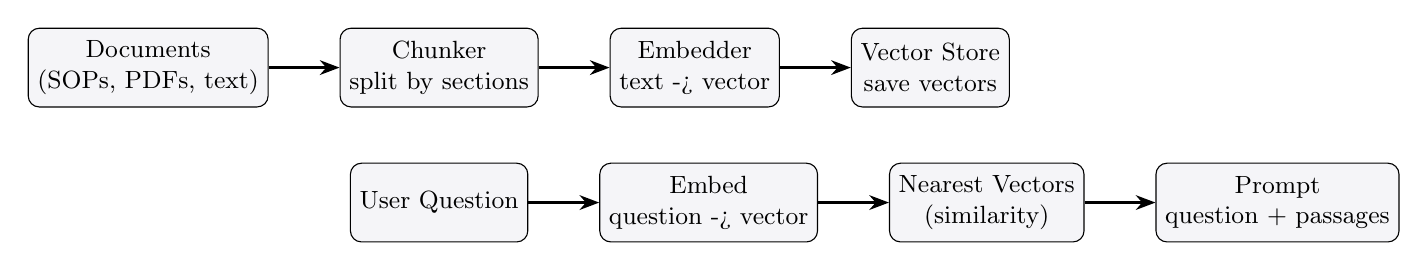
\begin{tikzpicture}[
  node distance=7mm and 9mm,
  stepbox/.style={draw, rounded corners, fill=softgray, minimum height=10mm, align=center, font=\small},
  arrow/.style={-{Stealth[length=2.5mm]}, thick}
]
  \node[stepbox] (doc) {Documents\\(SOPs, PDFs, text)};
  \node[stepbox, right=of doc] (chunk) {Chunker\\split by sections};
  \node[stepbox, right=of chunk] (emb) {Embedder\\text -> vector};
  \node[stepbox, right=of emb] (store) {Vector Store\\save vectors};
  \node[stepbox, below=of chunk] (query) {User Question};
  \node[stepbox, right=of query] (qemb) {Embed\\question -> vector};
  \node[stepbox, right=of qemb] (search) {Nearest Vectors\\(similarity)};
  \node[stepbox, right=of search] (prompt) {Prompt\\question + passages};
  \draw[arrow] (doc) -- (chunk);
  \draw[arrow] (chunk) -- (emb);
  \draw[arrow] (emb) -- (store);
  \draw[arrow] (query) -- (qemb);
  \draw[arrow] (qemb) -- (search);
  \draw[arrow] (search) -- (prompt);
\end{tikzpicture}
\end{center}

\textbf{Indexing path} (runs once per document):
\codefile{knowledge.ingest\_document()} in \codefile{backend/app/services/knowledge.py}
calls \codefile{chunker.chunk\_text()}, \codefile{embeddings.embed()}, and
\codefile{vector\_store.upsert()}.

\textbf{Query path} (runs per question): \codefile{knowledge.retrieve()} embeds the
question, asks the store for nearest chunks, \textbf{blends} the similarity score with
a keyword-overlap score (0.8/0.2), and returns \codefile{Citation} objects
(document, version, section, score, snippet).

\subsection{Chunking: why size matters}
Embeddings turn a chunk into one vector -- so a chunk that mixes five topics becomes a
mushy average. Our chunker (\codefile{services/chunker.py}) splits on \emph{headings}
first (``SECTION 3: CUTTING PARAMETERS''), packs paragraphs up to $\approx$1200
characters with 150 characters of overlap between consecutive chunks, and records the
section name as metadata -- so citations can say ``SOP-MILL-001, Section 3.''

\layman{Like filing: don't stuff the whole manual into one folder. Cut it at chapter
boundaries so each folder is about one thing, and keep the chapter title on the tab.}

% ==================================================================
\section{Embeddings \& Vector Search}
% ==================================================================

\subsection{The concept}
An \textbf{embedding} is a list of numbers (a vector) that represents a text's
\emph{meaning}. Texts with similar meanings get vectors that point in similar
directions. The similarity of two texts is the \textbf{cosine} of the angle between
their vectors: 1.0 = identical meaning, 0.0 = unrelated.

\layman{Think of a map where every sentence is a city. ``How fast can I mill steel?''
and ``Roughing steel: 3000--5000 RPM'' are two streets in the same neighborhood;
``Employee parking policy'' is in another state. We find answers by searching the
neighborhood, not by reading every page.}

\subsection{Two providers, one interface}
\codefile{services/embeddings.py} defines an abstract
\codefile{BaseEmbeddings} with two implementations:
\begin{itemize}[nosep]
  \item \textbf{OpenAICompatibleEmbeddings} -- calls any \codefile{/v1/embeddings}
        endpoint (OpenAI, Azure, vLLM, Ollama). Production quality.
  \item \textbf{HashingEmbeddings} -- a zero-dependency offline fallback: it hashes
        each word/bigram into buckets to build a vector. It knows \emph{words}, not
        \emph{meaning}. Used in dev/tests so the whole system runs with no API key.
\end{itemize}

\layman{The real model understands that ``RPM'' and ``spindle speed'' are related.
The hashing fallback is a hyper-literal librarian: it only matches when you use the
same words. Both plug into the same socket, so switching is one line in \codefile{.env}.}

\subsection{Calibration: why we rescale hashing scores}
Real semantic models give meaningful matches cosine scores like 0.4--0.8, and garbage
around 0.1--0.2. Hashing vectors give meaningful matches around 0.25--0.33 and garbage
0.10--0.15 -- a \emph{compressed band}. A fixed threshold like 0.25 would behave
completely differently on the two providers. So in \codefile{knowledge.retrieve()} we
rescale the hashing band onto [0,1] (a linear map, like converting Celsius to
Fahrenheit), so one threshold works everywhere. The lesson generalizes: \textbf{when
swapping models, recalibrate thresholds -- score scales are model-specific, not
universal}.

\subsection{Vector stores}
\codefile{services/vector\_store.py} offers:
\begin{itemize}[nosep]
  \item \textbf{NumpyVectorStore} -- exact cosine search, in-memory, rebuilt from the
        database at startup. Perfect for one server and a few thousand chunks.
  \item \textbf{ChromaVectorStore} -- optional persistent ANN store
        (\codefile{pip install .[chroma]}) for larger corpora.
\end{itemize}
Both implement \codefile{upsert / delete\_document / search / count} -- the rest of the
system never knows which is running. \emph{Program to an interface} is the pattern.

\subsection{Hybrid retrieval}
Dense similarity misses exact keywords (``h6 tolerance''), and keyword matching misses
paraphrases. We do both and blend: $\text{final} = 0.8 \times \text{dense} + 0.2
\times \text{keyword overlap}$. This is called \textbf{hybrid search} and is what real
production RAG systems do.

% ==================================================================
% Part 2: LLMs, structured output, planning, rules, inspection,
%         human-in-the-loop, security, deployment, glossary.
% Included from concepts_guide.tex -- do not compile directly.
% ==================================================================

% ==================================================================
\section{LLMs, Structured Output \& the Planner}
% ==================================================================

\subsection{The concept of an LLM gateway}
Different providers (OpenAI, Azure, vLLM, Ollama) all speak a nearly identical
``chat completions'' dialect. \codefile{services/llm.py} wraps that dialect behind one
interface, so the planner/Q\&A/inspection code never says ``OpenAI'' -- it says
``\codefile{llm.complete\_json(...)}''. Swapping providers is a \codefile{.env} edit,
not a code edit.

\subsection{Structured output: the single most important LLM trick}
A plan must be \emph{data} (operations, machines, parameters), not an essay -- data can
be validated, stored, versioned, and shown in a UI. The trick:
\begin{enumerate}[nosep]
  \item Define a Pydantic schema (\codefile{services/plan\_schema.py}):
        \codefile{GeneratedPlan} with \codefile{operations[]}, each having
        \codefile{op\_number, machine, tooling, parameters\dots}.
  \item Instruct the model: ``Output ONLY JSON matching this shape.''
  \item Parse the reply, extract the JSON (even from markdown fences),
        \emph{validate against the schema}.
  \item If validation fails, send the errors back: ``Your JSON failed validation
        because X. Return corrected JSON only.'' (One bounded retry.)
\end{enumerate}

\begin{center}
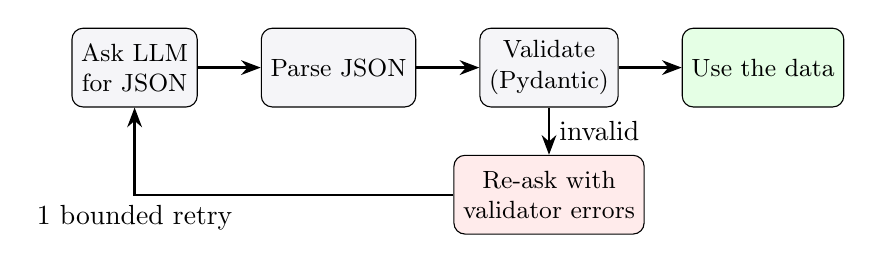
\begin{tikzpicture}[
  node distance=6mm and 8mm,
  stepbox/.style={draw, rounded corners, fill=softgray, minimum height=10mm, align=center, font=\small},
  err/.style={stepbox, fill=red!8},
  arrow/.style={-{Stealth[length=2.5mm]}, thick}
]
  \node[stepbox] (ask) {Ask LLM\\for JSON};
  \node[stepbox, right=of ask] (parse) {Parse JSON};
  \node[stepbox, right=of parse] (val) {Validate\\(Pydantic)};
  \node[stepbox, right=of val, fill=green!10] (ok) {Use the data};
  \node[err, below=of val] (retry) {Re-ask with\\validator errors};
  \draw[arrow] (ask) -- (parse);
  \draw[arrow] (parse) -- (val);
  \draw[arrow] (val) -- (ok);
  \draw[arrow] (val) -- node[right]{invalid} (retry);
  \draw[arrow] (retry) -| node[below]{1 bounded retry} (ask);
\end{tikzpicture}
\end{center}

\layman{It's a tax form. You don't accept a free-text letter; you reject the form,
circle the wrong fields, and hand it back once. After one retry you escalate to a
human. This converts ``the model said something'' into ``the data passed the schema.''}
This loop lives in \codefile{llm.complete\_json()}.

\subsection{The planner pipeline}
\codefile{services/planner.py} orchestrates five steps:
\begin{enumerate}[nosep]
  \item \textbf{Retrieve} knowledge for the part (SOPs, routings, standards, lessons)
        $\rightarrow$ numbered context blocks \codefile{[K1]..[Kn]}.
  \item \textbf{Prompt} the LLM: requirements + context + ``cite the [Kn] you use.''
  \item \textbf{Structured generation} via \codefile{complete\_json}.
  \item \textbf{Rule validation} (\S\ref{sec:rules}); if errors, one repair round with
        the rule violations fed back to the model.
  \item \textbf{Grounding report}: count operations carrying citations; scan for
        numeric specs (``0.1 mm'', ``1800 RPM'') that appear in \emph{no} retrieved
        chunk $\rightarrow$ flagged as \textbf{unverified claims} shown to the engineer.
\end{enumerate}

\subsection{The refusal gate: when the assistant says ``I don't know''}
\label{sec:refusal}
The Q\&A endpoint refuses to answer when retrieval shows nothing relevant. Two checks
(\codefile{services/qa.py}):
\begin{enumerate}[nosep]
  \item \textbf{Absolute floor}: the best chunk's calibrated score is below a
        threshold -- nothing even came close.
  \item \textbf{Separation}: compare the best chunk's score to the \emph{average}
        score across the whole corpus for this query. A question the corpus can
        answer produces one neighborhood clearly above the background (separation
        $\gg 1$); a question about nothing in the corpus scores uniformly -- nothing
        stands out (separation $\approx 1$) $\Rightarrow$ refuse.
\end{enumerate}
\layman{Before answering, the assistant glances at the whole library: if one book
lights up for this question, answer from it; if everything is equally dim, say
``this isn't in the library'' instead of improvising. That self-comparison makes the
threshold work for \emph{any} embedding model without manual tuning.}

\subsection{The offline FakeLLM}
\codefile{FakeLLM} returns deterministic canned JSON (plan, inspection, or Q\&A,
routed by prompt markers). This is not a toy: it makes the \emph{entire product} --
auth, RAG, planning, validation, approval, UI -- testable and demonstrable with zero
API cost, and makes the 29 automated tests hermetic (no network flakiness).

% ==================================================================
\section{Deterministic Validation: The Rule Engine}\label{sec:rules}
% ==================================================================

\subsection{The concept}
LLMs propose; rules dispose. After generation, plain Python code re-checks the plan
against plant master data. No probability involved -- the same input always yields the
same verdict. This is how you get \emph{auditability}: ``why was this plan rejected?''
has a precise answer: ``rule MACH\_FORBIDDEN: milling is not allowed on CNC Lathe-1.''

\layman{The AI is a talented intern writing the plan; the rule engine is the grumpy
but reliable inspector with the checklist who stamps it. Interns get better with
feedback; the checklist never gets tired or creative.}

\subsection{What the rules check}
Rules live in \textbf{YAML} (\codefile{data/rulepacks/shop\_rules.yaml}) so process
engineers can edit them \emph{without touching code}:
\begin{itemize}[nosep]
  \item \textbf{Structural}: op numbers strictly increasing, every op has a machine,
        an inspection plan exists, checkpoints present (warnings).
  \item \textbf{Machine capability}: machine must exist in approved master data
        (\codefile{MACH\_UNKNOWN}); process must be permitted there
        (\codefile{MACH\_FORBIDDEN}); parameters within the approved list.
  \item \textbf{Material}: forbidden processes per material; required notes
        (``material certification'') present -- else warning.
  \item \textbf{Quantity policy}: orders $\leq$10 pcs require 100\% visual inspection
        in the plan (\codefile{QTY\_INSPECT}).
\end{itemize}

\subsection{The repair loop}
If errors exist, the planner sends them back to the LLM once: ``fix these rule
violations and return the full corrected JSON.'' If it still fails, the plan is saved
\emph{with its errors visible} -- never silently fixed, never silently accepted. The
engineer sees \codefile{RuleValidationReport} with rule IDs, severity, and messages.

\begin{center}
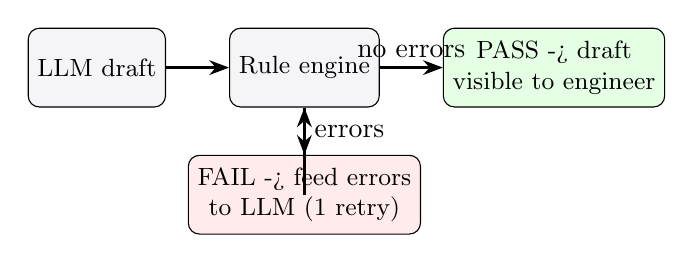
\begin{tikzpicture}[
  node distance=6mm and 8mm,
  stepbox/.style={draw, rounded corners, fill=softgray, minimum height=10mm, align=center, font=\small},
  arrow/.style={-{Stealth[length=2.5mm]}, thick}
]
  \node[stepbox] (gen) {LLM draft};
  \node[stepbox, right=of gen] (val) {Rule engine};
  \node[stepbox, right=of val, fill=green!10] (pass) {PASS -> draft\\visible to engineer};
  \node[stepbox, below=of val, fill=red!8] (fail) {FAIL -> feed errors\\to LLM (1 retry)};
  \draw[arrow] (gen) -- (val);
  \draw[arrow] (val) -- node[above]{no errors} (pass);
  \draw[arrow] (val) -- node[right]{errors} (fail);
  \draw[arrow] (fail) -| (val);
\end{tikzpicture}
\end{center}

% ==================================================================
\section{Vision Inspection: Quality Gate + VLM}
% ==================================================================

\subsection{The concept}
A \textbf{VLM} (vision-language model) reads an image plus a text prompt and answers
in text: ``there is a scratch in the upper-left quadrant, confidence 0.8.'' But models
are only as good as their input -- a blurry, dark, or glared photo produces confident
nonsense. So before the VLM ever runs, deterministic \textbf{image quality metrics}
decide whether the image is analyzable at all.

\subsection{The quality gate (pure classical CV, no AI)}
\codefile{services/inspection.py::assess\_quality()} computes four metrics with
OpenCV:
\begin{itemize}[nosep]
  \item \textbf{Resolution}: width/height minimums (can we see detail at all?).
  \item \textbf{Brightness}: mean pixel intensity within bounds (not pitch-black,
        not washed out).
  \item \textbf{Sharpness}: variance of the Laplacian -- blur smears edges, which
        lowers this variance dramatically (the classic blur detector).
  \item \textbf{Glare}: fraction of near-saturated pixels (specular reflections
        hide the surface underneath).
\end{itemize}
Failed gate $\Rightarrow$ verdict \textbf{inconclusive} with the exact failed checks
listed. \emph{``We cannot judge this image'' is the honest answer} -- challenge \#2 from
the project brief, solved with arithmetic instead of hope.

\layman{The bouncer checks ID before letting anyone into the club. Dark, blurry, or
glared photos are turned away at the door with a reason -- they never reach the
(overconfident) AI inside.}

\subsection{The analysis pipeline}

\begin{center}
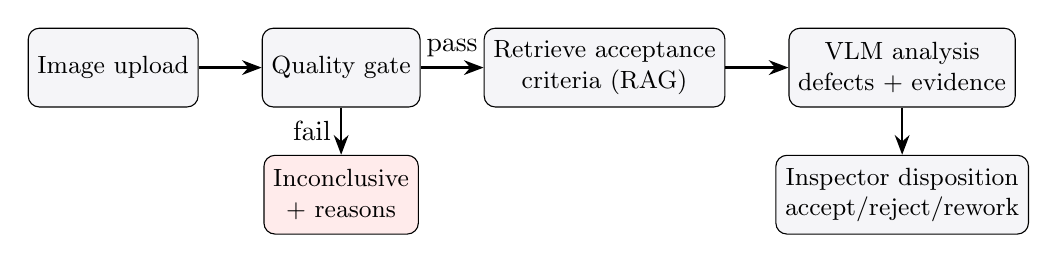
\begin{tikzpicture}[
  node distance=6mm and 8mm,
  stepbox/.style={draw, rounded corners, fill=softgray, minimum height=10mm, align=center, font=\small},
  arrow/.style={-{Stealth[length=2.5mm]}, thick}
]
  \node[stepbox] (img) {Image upload};
  \node[stepbox, right=of img] (gate) {Quality gate};
  \node[stepbox, right=of gate] (ctx) {Retrieve acceptance\\criteria (RAG)};
  \node[stepbox, right=of ctx] (vlm) {VLM analysis\\defects + evidence};
  \node[stepbox, below=of gate, fill=red!8] (incon) {Inconclusive\\+ reasons};
  \node[stepbox, below=of vlm] (human) {Inspector disposition\\accept/reject/rework};
  \draw[arrow] (img) -- (gate);
  \draw[arrow] (gate) -- node[above]{pass} (ctx);
  \draw[arrow] (gate) -- node[left]{fail} (incon);
  \draw[arrow] (ctx) -- (vlm);
  \draw[arrow] (vlm) -- (human);
\end{tikzpicture}
\end{center}

Note the second RAG use: before analysis we retrieve the \emph{visual acceptance
criteria} (e.g., QS-77: ``scratches $>$5mm on sealing faces = reject'') and paste them
into the VLM prompt -- so defect judgments reference plant policy, not model vibes.

\subsection{Calibrated thresholds and evidence}
Every defect carries a \textbf{confidence}. Below-threshold findings are kept but
marked \codefile{below\_threshold: true} -- shown to the human differently rather than
hidden. Each defect needs \textbf{evidence} (``linear mark consistent with handling,
does not catch fingernail'') -- because an inspector must be able to \emph{disagree}
with the AI, and the audit trail records who decided what.

% ==================================================================
\section{Human-in-the-Loop \& Traceability}
% ==================================================================

\subsection{The state machine}
Nothing generated is ever ``final''. A plan is a \textbf{state machine}
(\codefile{models.PlanStatus}, enforced in \codefile{routes/plans.py}):

\begin{center}
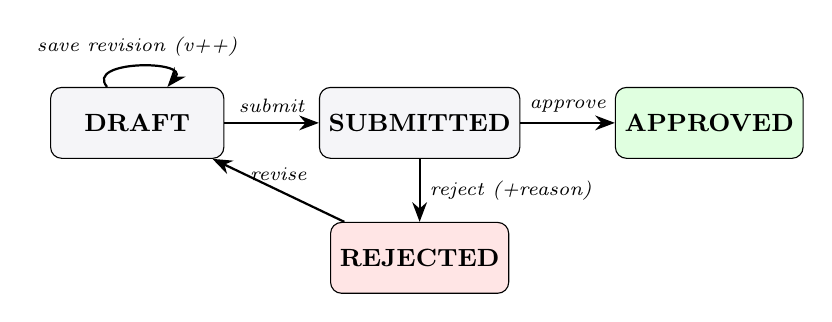
\begin{tikzpicture}[
  node distance=8mm and 12mm,
  st/.style={draw, rounded corners, fill=softgray, minimum width=22mm, minimum height=9mm, font=\small\bfseries},
  arrow/.style={-{Stealth[length=2.5mm]}, thick},
  lab/.style={font=\scriptsize\itshape}
]
  \node[st] (draft) {DRAFT};
  \node[st, right=of draft] (submitted) {SUBMITTED};
  \node[st, right=of submitted, fill=green!12] (approved) {APPROVED};
  \node[st, below=of submitted, fill=red!10] (rejected) {REJECTED};
  \draw[arrow] (draft) -- node[lab, above]{submit} (submitted);
  \draw[arrow] (submitted) -- node[lab, above]{approve} (approved);
  \draw[arrow] (submitted) -- node[lab, right]{reject (+reason)} (rejected);
  \draw[arrow] (rejected) -- node[lab, above]{revise} (draft);
  \draw[arrow] (draft) to[out=130, in=50, looseness=1.5] node[lab, above]{save revision (v++)} (draft);
\end{tikzpicture}
\end{center}

Illegal transitions are rejected by the API (you cannot approve a draft -- first it
must be submitted). Every transition writes an \codefile{Approval} row: who, what,
when, comment, and a \textbf{snapshot of the plan as it was reviewed}. The DB rejects
the write if a transition is invalid -- the database itself is the last line of defense.

\subsection{The audit trail}
Every meaningful action (plan generated, decision taken, disposition set, document
ingested) appends to \codefile{audit\_logs} with actor, action, target, and JSON
detail. Admins can read the tail via \codefile{/admin/audit}. This is the
``black box'' that answers ``who did what, when, and based on which sources'' -- the
traceability objective from the brief.

\subsection{Feedback: learning from corrections}
Every plan and inspection can be rated 1--5 with notes and structured corrections
(\codefile{feedback} table). Approving with edits, rejecting with reasons, accepting
or reworking parts -- all become \emph{training signal} for prompt/RAG improvements.
This is the ``Manufacturing Memory'' innovation: the system compounds the value of
every human decision instead of discarding it.

% ==================================================================
\section{Security \& Users}
% ==================================================================

\subsection{JWT authentication in plain words}
Login once $\Rightarrow$ server issues two signed tokens:
an \textbf{access token} (short-lived, 30 min, sent as \codefile{Authorization: Bearer
...} on every API call) and a \textbf{refresh token} (7 days, used once to get a new
pair, then invalidated -- ``rotation''). The server signs tokens with a secret key;
it never stores passwords in readable form (bcrypt hash). Anyone can \emph{read} a
token; nobody can \emph{forge} one without the secret.

\layman{Access token = a day pass stamped by the guard; refresh token = your
membership card that lets you get a new day pass at the desk -- once per card, so a
stolen card can't be reused silently.}

\subsection{Roles}
Three roles: \textbf{admin} (user management, audit), \textbf{engineer} (generate,
approve, inspect, ingest), \textbf{viewer} (read-only). Enforced by a dependency
(\codefile{require\_roles}) on each route; the first registered user becomes admin.

\subsection{Defense in depth (the challenges table, implemented)}
\begin{center}
\begin{tabular}{@{}p{4.6cm}p{9.5cm}@{}}
\toprule
\textbf{Threat} & \textbf{Mitigation in this codebase} \\
\midrule
Hallucinated advice & RAG + citations + schema-validated output + unsupported-claim scan + human approval \\
Bad images & Deterministic quality gate with explicit failure reasons \\
Rule violations & YAML rule packs + repair loop + never-silently-accept \\
Unauthorized access & JWT + roles + bcrypt + refresh rotation \\
Abuse & Per-IP rate limiting middleware \\
Lost accountability & Audit log + approval snapshots + versioned documents \\
Secret leakage & \codefile{.env} outside git; \codefile{.env.example} documents every key \\
\bottomrule
\end{tabular}
\end{center}

% ==================================================================
\section{Production Engineering Practices Used}
% ==================================================================

\begin{description}[leftmargin=0pt, style=unboxed, itemsep=2pt]
  \item[12-factor config.] Every knob is an environment variable with a safe default
      (\codefile{core/config.py}); no secrets in code; \codefile{.env.example} is the contract.
  \item[Error taxonomy.] One exception class per failure type
      (\codefile{core/errors.py}) mapped to HTTP codes; clients get
      \codefile{\{error: \{code, message\}\}} -- never a stack trace.
  \item[Structured logs + request IDs.] JSON logs with a request-id contextvar
      (\codefile{core/logging.py}, \codefile{core/middleware.py}); grep-able and
      traceable across services.
  \item[Health \& metrics.] \codefile{/health} reports provider and DB status;
      \codefile{/metrics} exposes Prometheus counters -- what a load balancer and a
      dashboard need.
  \item[Interface swappability.] LLM, embeddings, vector store are each behind a tiny
      abstract base -- providers are .env choices, not rewrites.
  \item[Hermetic tests.] 29 tests cover auth, ingestion, retrieval, refusal, planning,
      rules, inspection gate, dispositions, feedback, dashboard, audit -- all offline,
      deterministic, fast (seconds).
  \item[Containers.] \codefile{Dockerfile.backend/.frontend} +
      \codefile{docker-compose.yml / .prod.yml} give one-command deploys with
      Postgres, healthchecks, and an nginx reverse proxy with security headers.
\end{description}

% ==================================================================
\section{Glossary (Jargon $\rightarrow$ Plain Words)}
% ==================================================================

\begin{longtable}{@{}p{3.4cm}p{12.2cm}@{}}
\toprule
\textbf{Term} & \textbf{What it actually means} \\
\midrule
LLM & Large Language Model -- a neural network trained on text that predicts plausible continuations. Brilliant, occasionally wrong with total confidence. \\
VLM & The same idea for images: picture + question in, description out. \\
RAG & Retrieve relevant passages first, then have the LLM answer \emph{only from them}, citing them. \\
Embedding & A list of numbers representing a text's meaning; similar meaning = similar numbers (nearby vector). \\
Cosine similarity & $1 - $ angle between two vectors; 1 = same meaning, 0 = unrelated. \\
Vector store & A database that finds nearest vectors fast. \\
Chunk & A paragraph-sized piece of a document; the unit of retrieval and citation. \\
Token & A word-piece; how LLMs and embeddings split text (and how they charge you). \\
Prompt & The full text sent to the model: instructions + context + question. \\
System prompt & The standing instructions defining the model's role and rules. \\
Hallucination & The model inventing facts. Cured here by grounding, citations, refusal. \\
JSON schema & The exact required structure of an answer; used to force usable data out of the model. \\
Rule engine & Deterministic Python checks against plant master data; no AI involved. \\
Quality gate & Pre-AI arithmetic checks (blur/brightness/glare) that refuse unusable images. \\
Disposition & The human decision on a part: accept / reject / rework. \\
JWT & A signed token proving who you are; contains claims (user id, role, expiry). \\
bcrypt & A slow, salted password hash; passwords are never stored in plain text. \\
CORS & Browser rule for which websites may call the API; configured via env. \\
Rate limiting & Cap requests per minute per client to survive abuse or bugs. \\
ANN & Approximate Nearest Neighbor -- vector search that trades a little accuracy for a lot of speed. \\
Migration & A versioned change to the DB schema (Alembic); tables evolve without data loss. \\
Idempotent & Running it twice has the same effect as once (seed script, ingestion). \\
\bottomrule
\end{longtable}

\section*{How to study this codebase in one evening}
\begin{enumerate}[nosep]
  \item Read \codefile{backend/app/core/config.py} -- see every knob with its default.
  \item Read \codefile{services/knowledge.py} -- indexing and retrieval, 200 lines.
  \item Read \codefile{services/planner.py} -- the 5-step pipeline and its prompts.
  \item Read \codefile{services/rules.py} + \codefile{data/rulepacks/shop\_rules.yaml}
        -- how plants encode expertise.
  \item Read \codefile{services/inspection.py::assess\_quality} -- 40 lines of honest
        computer vision.
  \item Run \codefile{pytest} and read the tests -- they are executable specifications.
  \item Click through the UI with the demo account and watch the API logs stream.
\end{enumerate}

\noindent\emph{The core lesson of this architecture: LLMs are used where language
matters, arithmetic where truth matters, and humans where judgment matters -- and
every layer can show its work.}


\end{document}
